\documentclass[border=10pt]{standalone}
\usepackage{tikz}

\begin{document}
    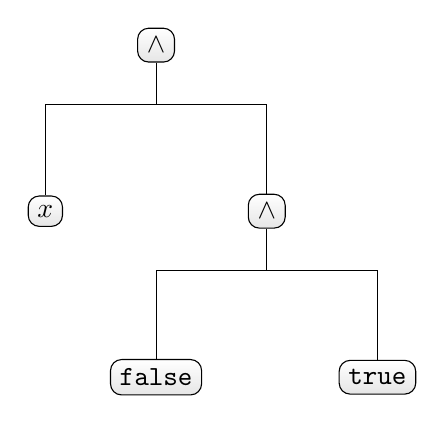
\begin{tikzpicture}[sibling distance=8em,
        level distance=6em,
        edge from parent/.style={
            draw,
            edge from parent path={
                (\tikzparentnode.south) -- ++(0,-1.5em) -| (\tikzchildnode.north)
            }
        },
        every node/.style = {shape=rectangle, rounded corners,
        draw, align=center,
        top color=white, bottom color=gray!20}]]
        
        \node {$\land$}
        child { node {$x$} }
        child { node {$\land$}
            child { node {\texttt{false}} }
            child { node {\texttt{true}} }
        };
    \end{tikzpicture}
\end{document}